\section{Análisis de Resultados}

El análisis de resultados permitió evidenciar que las arquitecturas Kappa y Delta presentan características, 
ventajas y limitaciones diferenciadas, las cuales deben ser consideradas cuidadosamente según el contexto de aplicación. \newline

La arquitectura Kappa demostró ser altamente eficiente para el procesamiento en tiempo real, logrando latencias inferiores al segundo en más del 80 \% de los casos. 
Esta capacidad la posiciona como la opción más adecuada en escenarios donde la reacción inmediata es crítica, 
como en el monitoreo de pacientes en unidades de cuidados intensivos o emergencias. 
No obstante, esta eficiencia viene acompañada de un mayor consumo de recursos, 
una complejidad operativa superior y una necesidad considerable de almacenamiento, 
debido a su dependencia de Kafka como fuente de verdad. \newline

Por otro lado, la arquitectura Delta evidenció una mayor escalabilidad y una mejor eficiencia en el uso de recursos, 
en particular en almacenamiento y transferencia de datos, gracias al uso de formatos columnar como Parquet y almacenamiento en Object Storage. 
Sin embargo, sus tiempos de latencia (aunque estables) alcanzaron valores promedio de alrededor de 180 segundos, 
lo que la hace inadecuada para casos que requieren inmediatez. Aun así, esta latencia puede considerarse aceptable en contextos como el monitoreo ambulatorio, 
donde las decisiones clínicas no dependen de una reacción instantánea. \newline

En cuanto a throughput, Delta logró duplicar la capacidad de ingesta de Kappa, 
procesando hasta 1300 registros por segundo frente a los 790 de Kappa. 
Asimismo, logró completar el 100 \% de la carga de datos, a diferencia de Kappa, 
que presentó fallos por limitaciones en el uso de disco durante el despliegue. \newline

Se puede ver que se desde la perspectiva del principio SCV, Kappa elige Volumen y Velocidad,
mientras que Delta elige Volumen y Consistencia. Esto debido a las características de las tecnologías usadas. 
Kappa hace uso extensivo de Kafka que le permite tener una mínima latencia 
y Delta utiliza Paimon que permite tener transacciones ACID y ofrece consistencia como la base de sus capacidades.

\newpage

Desde la perspectiva económica, el despliegue de Delta implicó un costo 36 \% menor que el de Kappa. 
Esta diferencia se debe principalmente a la menor necesidad de almacenamiento persistente y al menor tráfico de red requerido.\newline

Dado lo anterior, la elección entre Kappa y Delta dependerá del caso de uso específico.

Para un sistema de salud integral, una estrategia híbrida que combine ambas arquitecturas se perfila como una solución óptima. 
En este enfoque, Delta puede actuar como fuente de verdad y repositorio histórico, 
mientras que un subsistema basado en Kappa podría operar en paralelo para los casos donde la baja latencia sea un requerimiento indispensable. \newline

Esta estrategia se asemeja conceptualmente a la arquitectura Lambda, 
aunque enfocada en el procesamiento continuo de datos y utilizando tecnologías actuales como Doris, 
que permite consultas federadas sobre los datos almacenados en ambas arquitecturas; 
y Kafka que permite el ruteo de mensajes a ambos sistemas a la vez paraque cada uno lo procese a la velocidad que pueda.

\begin{figure}[h]
    \makebox[\textwidth]{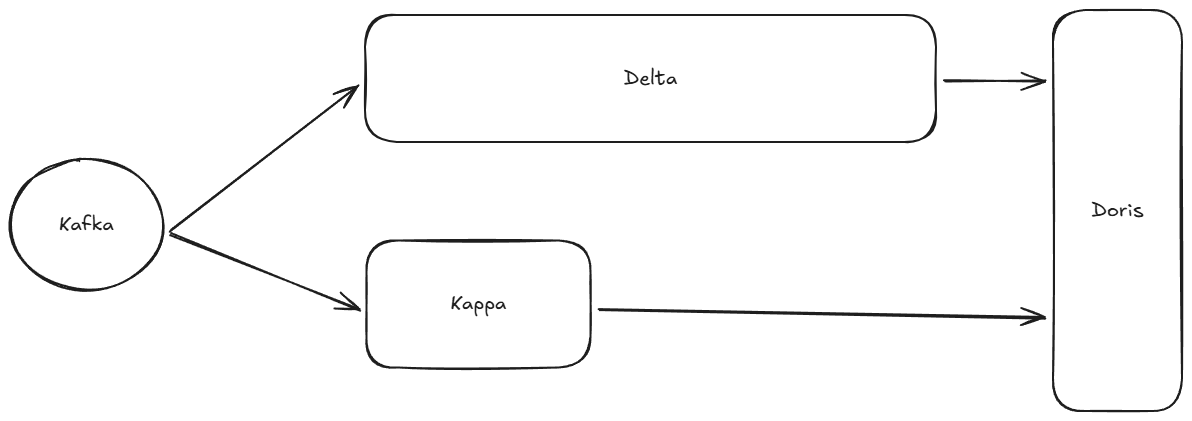
\includegraphics[width=\paperwidth]{resultados/combine.png}}
    \caption{Arquitectura combinada de un sistema de salud integral} 
    \label{fig:des_arquitectura_combinada}
\end{figure}